\documentclass[border=8pt]{standalone}
\usepackage[utf8]{inputenc}
\usepackage{nacal}
\usepackage{tikz}
\usepackage{tikz-3dplot}
\usetikzlibrary{calc,angles,positioning,intersections,quotes,decorations.markings,arrows.meta,decorations.pathreplacing}
\usepackage{tkz-euclide}
\def\Datos{green!40!gray}
\def\Ajuste{blue!50!red}
\def\Residuo{black!25!gray}
\def\Regresor{blue!75!white}
\def\Base{orange!80!black}
\def\Sistem{blue!50!black}
\tikzset{vector/.style={-{Stealth[length=3mm, width=2mm]},very thick},
         basevec/.style={-{Stealth[length=2.2mm, width=1.6mm]},thick,\Base},
         guide/.style={dashed,thin,gray}}

\begin{document}
  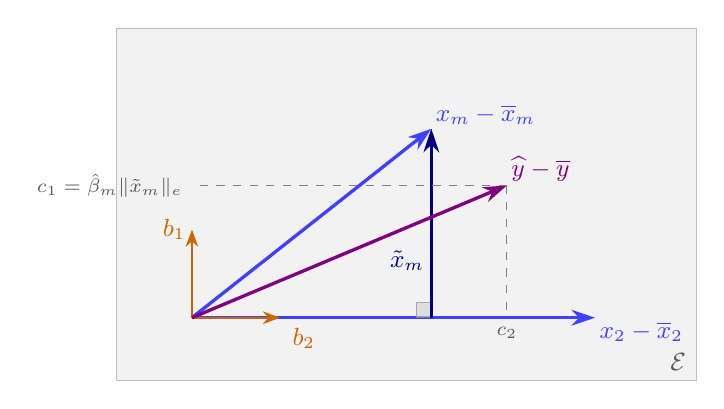
\begin{tikzpicture}[scale=1.6]
    \coordinate (O)  at (0,0);
    \coordinate (X2) at (3.2,0);        % otro regresor en desviaciones
    \coordinate (Xm) at (1.9,1.5);      % x_m en desviaciones
    \coordinate (Xp) at (1.9,0);        % su proyección sobre el otro regresor
    \coordinate (Tm) at (0,1.5);        % parte propia, trasladada al origen
    \coordinate (A)  at (2.5,1.05);     % ajuste en desviaciones
    \coordinate (Ax) at (2.5,0);
    \coordinate (Ay) at (0,1.05);
    % el plano E
    \fill[gray!10,draw=gray!50,very thin] (-0.6,-0.5) rectangle (4.0,2.3);
    \node[gray!70!black,anchor=south east,font=\small] at (4.0,-0.5) {$\mathcal E$};
    % regresores en desviaciones
    \draw[vector,\Regresor] (O) -- (X2) node[anchor=north west,font=\small,inner sep=1pt] {$\boldsymbol x_2-\boldsymbol{\mathop{\overline x}}_2$};
    \draw[vector,\Regresor] (O) -- (Xm) node[anchor=south west,font=\small,inner sep=1pt] {$\boldsymbol x_m-\boldsymbol{\mathop{\overline x}}_m$};
    \draw[guide] (Xm) -- (Xp);
    \tkzMarkRightAngle[size=.12,gray,very thin,fill=lightgray!70,opacity=0.6](O,Xp,Xm)
    % parte propia
    \draw[vector,\Sistem] (Xp) -- (Xm) node[pos=0.3,anchor=east,font=\small,inner sep=2pt] {$\tilde{\boldsymbol x}_m$};
    % base adaptada: b1 sobre la parte propia, b2 sobre el otro regresor
    \draw[basevec] (O) -- (0,0.7) node[anchor=east,font=\small,inner sep=2pt] {$\boldsymbol b_1$};
    \draw[basevec] (O) -- (0.7,0) node[anchor=north,font=\small,xshift=3mm] {$\boldsymbol b_2$};
    % ajuste en desviaciones y sus coordenadas
    \draw[vector,\Ajuste] (O) -- (A) node[anchor=south west,font=\small,inner sep=1pt] {$\boldsymbol{\mathop{\widehat y}}-\boldsymbol{\mathop{\overline y}}$};
    \draw[guide] (A) -- (Ax); \draw[guide] (A) -- (Ay);
    \node[font=\scriptsize,gray!70!black,anchor=north] at (Ax) {$c_2$};
    \node[font=\scriptsize,gray!70!black,anchor=east] at (Ay) {$c_1=\hat\beta_m\Vert\tilde{\boldsymbol x}_m\Vert_e$};
  \end{tikzpicture}
\end{document}
